\section{Auswertung}
\label{sec:Auswertung}
Alle aufgenommenen Messwerte sind in \autoref{sec:anhang} zu finden.
\subsection{Bestimmung der Absorptionskoeffizienten von Blei und Zink unter Einfluss
von Gamma-Strahlung}

Es wird als Strahlungsquelle Cäsium-137 verwendet, dessen Verhältnis der 
Quantenenergie zur Ruheenergie des Elektrons $\epsilon = 1,295$ beträgt.\\

\subsubsection*{Absorptionskurve}
Ohne Abschirmung wird eine Aktivität von $3,14 \; \mathrm{1/s}$ gemessen.
Die Ausgleichsgeraden wurde mit der Regressionsformel 
\begin{equation*}
  \mathrm{\ln}(N(D)) = - \mu D + \mathrm{\ln}(N_0)
  \label{eq:linreg}
\end{equation*}
erstellt.\\
\begin{figure}[H]
  \centering
  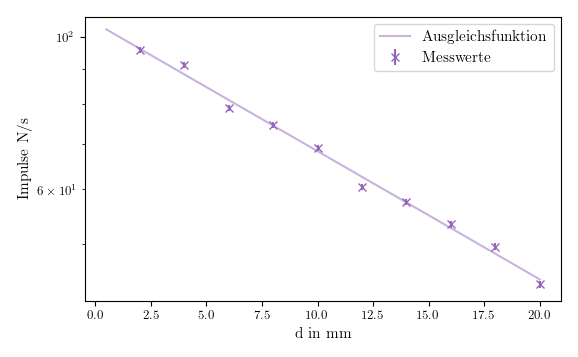
\includegraphics{content/verzweiflung.png}
  \caption{Die Messwerte der Impulsrate N in Abhängigkeit der 
  Schichtdicke d der Zinkabsorber halblogarithmisch aufgetragen und an eine lineare Funktion gefitted.}
  \label{fig:verzweiflung}
\end{figure}
\begin{figure}[H]
  \centering
  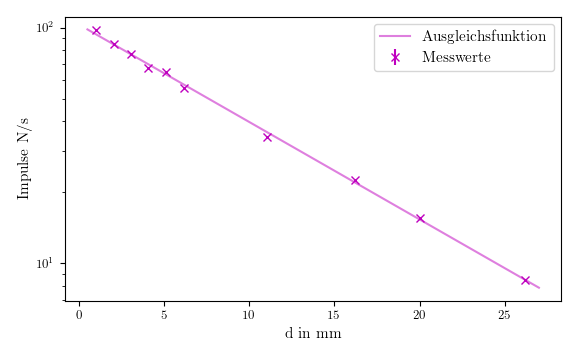
\includegraphics{content/pain.png}
  \caption{Die Messwerte der Impulsrate N in Abhängigkeit der 
  Schichtdicke d der Bleiabsorber halblogarithmisch aufgetragen und an eine lineare Funktion gefitted.}
  \label{fig:pain}
\end{figure}
In \autoref{fig:verzweiflung} und  \autoref{fig:pain} ist die graphische Darstellung der Berechnungen gemeinsam mit den 
gemessenen Werten aufgetragen. Der Betrag der Steigung der Ausgleichsgerade stellt hier den Absorptionskoeffizienten $\mu$ dar,
der y-Achsenabschnitt N(0) Es ergeben sich die Parameter 
\begin{eqnarray}
  \mu_{Zn} &=&  43,1 \pm 1,3\,  \mathrm{m^-1} \nonumber \\
  N(0)_{Zn} &=& 4,6 \pm 0,2 \, \mathrm{s^-1} \nonumber
\end{eqnarray}
für das Absorbermaterial Zink und 
\begin{eqnarray}
  \mu_{Pb} &=&  95,2 \pm 1,3 \,  \mathrm{m^-1} \nonumber \\
  N(0)_{Pb} &=& 4,7 \pm 0,2 \, \mathrm{s^-1} \nonumber
\end{eqnarray}
für Blei. \\



%\subsubsection*{Vergleich zwischen theoretisch und experimentiell bestimmten Werten}
%Alle Ergebnisse aus xxx und xxx sind zum Vergleich mit den theoretisch ermittelten Werten
%in \autoref{tab:vgl} aufgeführt. Die Theoriewerte wurden durch xxx berechnet.
%Der Vergleich zeigt, dass xxx.
%
%\begin{table}
%  \centering
%  \begin{tabular}{c c c}
%    \toprule
%     & Zink & Blei \\
%    \midrule
%      $\mu$ / \mathrm{m^-1} & xxx & xxx \\
%      N(0) / \mathrm{s^-1} & xxx & xxx  \\
%    \bottomrule
%  \end{tabular}
%  \caption{Absorptionskoeffizient $\mu$ und $N_0$ für xxx und xxx.}
%  \label{tab:vgl}
%\end{table}


\subsection{Bestimmung der Maximalenergie des verwendeten Beta-Strahlers}
\subsubsection*{Absorptionskurve}
Erneut wird eine Absorptionskurve aufgenommen. Nun werden als $\beta$-Strahler Technetium
und als Absorbermaterial Aluminium verwendet. 
Ohne Abschirmung wird eine Aktivität von $0,67 \; \mathrm{1/s}$ gemessen.
Die gemessenen Werte werden halblogarithmisch an \autoref{eq:linreg} gefitted und mit der Ausgleichsgeraden
in \autoref{fig:beta} graphisch dargestellt.\\
Mit der Formel
\begin{equation*}
  R_{\max} = \frac{m_2 - m_1}{b_1 - b_2}
\end{equation*}
kann der Schnittpunkt $R_{\max}$ der Ausgleichsgeraden ermittelt werden.\\
Die x-Koordinate dessen kennzeichnet multipliziert mit der Dichte von Aluminium \cite{aludichte} die maximale Reichweite, welche 
zur Berechnung der maximalen Energie mit \eqref{energie} benötigt wird. \\
Mit 
\begin{equation*}
  R_{\max} = 0,26 \pm 0,25 \; \mathrm{\frac{kg}{m^2}}   % maximale Reichweite Beta:  -0.26+/-0.25
\end{equation*}
ergibt sich 
\begin{equation*}
  E_{\max} = 0,19 \pm 0,5 \; \mathrm{MeV}    % maximale Energie Beta:  0.19452504787567537
\end{equation*}
für die maximale Energie.

\begin{figure}[H]
  \centering
  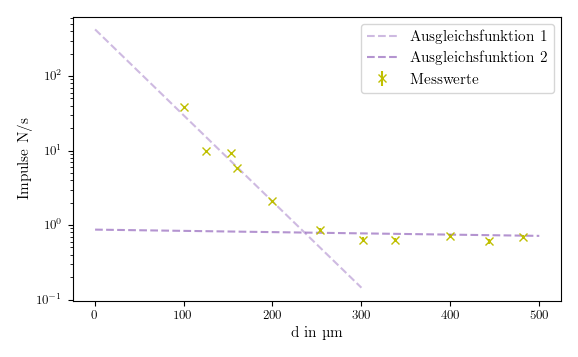
\includegraphics{content/zeitdruck.png}
  \caption{Die Messwerte der Impulsrate N in Abhängigkeit der 
  Schichtdicke d eines Aluminiumabsorbers halblogarithmisch aufgetragen und in den Plateaubereichen jeweils an eine lineare Funktion gefitted.}
  \label{fig:beta}
\end{figure}
